\documentclass[12pt]{fphw}

% Template-specific packages
\usepackage[utf8]{inputenc} % Required for inputting international characters
\usepackage[T1]{fontenc} % Output font encoding for international characters
\usepackage{mathpazo} % Use the Palatino font
\usepackage{graphicx} % Required for including images
\usepackage{booktabs} % Required for better horizontal rules in tables
\usepackage{listings} % Required for insertion of code
\usepackage{enumerate} % To modify the enumerate environment

%%%%%%%%%%%%%%%%%%%%%%%%%%%%%%%%%%

\usepackage[english]{babel}
\usepackage{amsmath}
\usepackage{graphicx}
\usepackage{float}
\usepackage[colorinlistoftodos]{todonotes}

\usepackage{xcolor}

\setlength{\parindent}{0em}

\begin{document}
\title{Travaux dirigés } % Assignment title
\author{Letao WANG}
\begin{titlepage}

\newcommand{\HRule}{\rule{\linewidth}{0.5mm}} % Defines a new command for the horizontal lines, change thickness here

\center % Center everything on the page
 
%----------------------------------------------------------------------------------------
%	HEADING SECTIONS
%----------------------------------------------------------------------------------------

\textsc{\large UFR Mathématiques et Informatique }\\[1.5cm] % Name of your university/college

\includegraphics[scale=.2]{logo_u-paris_tex_regular.png}\\[1cm] % Include a department/university logo - this will require the graphicx package
\textsc{\Large Algorithmique avancée}\\[0.5cm] % Major heading such as course name
\textsc{\large IF05X040}\\[0.5cm] % Minor heading such as course title

%----------------------------------------------------------------------------------------
%	TITLE SECTION
%----------------------------------------------------------------------------------------

\HRule \\[0.4cm]
{ \huge \bfseries Travaux Dirigés 6-7}\\[0.4cm] % Title of your document
\HRule \\[1.5cm]
 
%----------------------------------------------------------------------------------------
%	AUTHOR SECTION
%----------------------------------------------------------------------------------------

\begin{minipage}{0.4\textwidth}
\begin{flushleft} \large
\emph{Prof: }Nicolas \textsc{Loménie }\\
\emph{Author: }Letao \textsc{Wang}\\
\end{flushleft}

\end{minipage}\\[2cm]

% If you don't want a supervisor, uncomment the two lines below and remove the section above
%\Large \emph{Author:}\\
%John \textsc{Smith}\\[3cm] % Your name

%----------------------------------------------------------------------------------------
%	DATE SECTION
%----------------------------------------------------------------------------------------

{\large \today}\\[2cm] % Date, change the \today to a set date if you want to be precise

\vfill % Fill the rest of the page with whitespace

\end{titlepage}

%%%%%%%%%%%%%%%%%%%%%%%%%%%%%%%%%%%%%%%%

%----------------------------------------------------------------------------------------
%	ASSIGNMENT CONTENT
%----------------------------------------------------------------------------------------

\part*{Partie exercices}
\section*{Exercice 2.7.}
\begin{problem}
Déterminer un arbre couvrant de poids minimal pour le graphe de la
figure 2.3
\end{problem}
\subsection*{Réponse}

On peut utiliser l'algo de Prim et Kruskal, les resultat sont meme,
le poids minimal est 12.

\section*{Exercice 2.8.}
\begin{problem}
On considère un graphe valué G et un ensemble U de sommets. Proposer
un algorithme qui détermine un arbre couvrant de poids minimal parmi ceux tels que tous les sommets de U sont des feuilles.\\
Démontrer sa validité et préciser sa complexité.
\end{problem}
\subsection*{Réponse}

\section*{Exercice 2.9.}
\begin{center}
	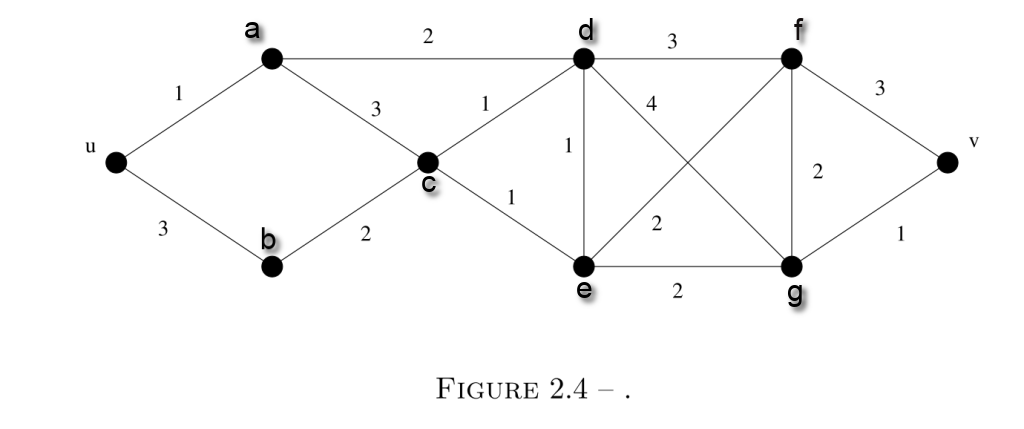
\includegraphics[width=1\columnwidth]{Figure2.4.png} % Example image
\end{center}
\subsection*{Réponse}
\begin{center}
l’algorithme de Dijkstra\\
	\begin{tabular}{l l l l l l l l l l}
		\toprule
		\textit{Sommet} & u & a & b & c & d &e & f & g & v\\
		\midrule
		Distance &  \textcolor{red}{0} & 1 &3 & $\infty$ & $\infty$  & $\infty$  & $\infty$  & $\infty$  & $\infty$  \\
		Distance &  \textcolor{red}{0} & \textcolor{red}{1} &3 & 4 & 3  & $\infty$  & $\infty$  & $\infty$  & $\infty$  \\
		Distance &  \textcolor{red}{0} & \textcolor{red}{1} &\textcolor{red}{3} & 4 & \textcolor{red}{3}  & 4  & 6  & 7  & $\infty$  \\
		Distance &  \textcolor{red}{0} & \textcolor{red}{1} &\textcolor{red}{3} & \textcolor{red}{4} & \textcolor{red}{3}  & \textcolor{red}{4}  & 6  & 6  & $\infty$  \\
		Distance &  \textcolor{red}{0} & \textcolor{red}{1} &\textcolor{red}{3} & \textcolor{red}{4} & \textcolor{red}{3}  & \textcolor{red}{4}  & \textcolor{red}{6}  & \textcolor{red}{6}  & 7  \\
		Distance &  \textcolor{red}{0} & \textcolor{red}{1} &\textcolor{red}{3} & \textcolor{red}{4} & \textcolor{red}{3}  & \textcolor{red}{4}  & \textcolor{red}{6}  & \textcolor{red}{6}  & \textcolor{red}{7}  \\
		\bottomrule
	\end{tabular}
\end{center}

\section*{Exercice 2.10}
\begin{problem}
A partir de l’algorithme de Dijkstra, construire un algorithme qui
détermine le diamètre de chaque composante connexe d’un graphe. Quelle en est la
complexité ?
\end{problem}
\subsection*{Réponse}

On fait l'algo Dijkstra pour tous les sommets  dans chaque composante connexe, retourner le plus grand nombre.

Complexity : n * algo Dijkstra ( on considere c'est $O(m + n log n)$  à l’aide de tas de Fibonacci) \\

Donc c'est $ O(n(m+n log n))$

\section*{Exercice 3.1.}
\subsection*{Réponse}
\begin{center}
	\begin{tabular}{l l l l}
		\toprule
		\textit{} & G1 & G2 & G3 \\
		\midrule
		Chemin eulérien & true & true & false\\
		Cycle eulérien & false & true & false\\
		Chemin hamiltonien & true & false & true\\
		Cycle hamiltonien & true & false & false\\
		\bottomrule
	\end{tabular}
\end{center}

\section*{Exercice 3.2.}

\begin{center}
	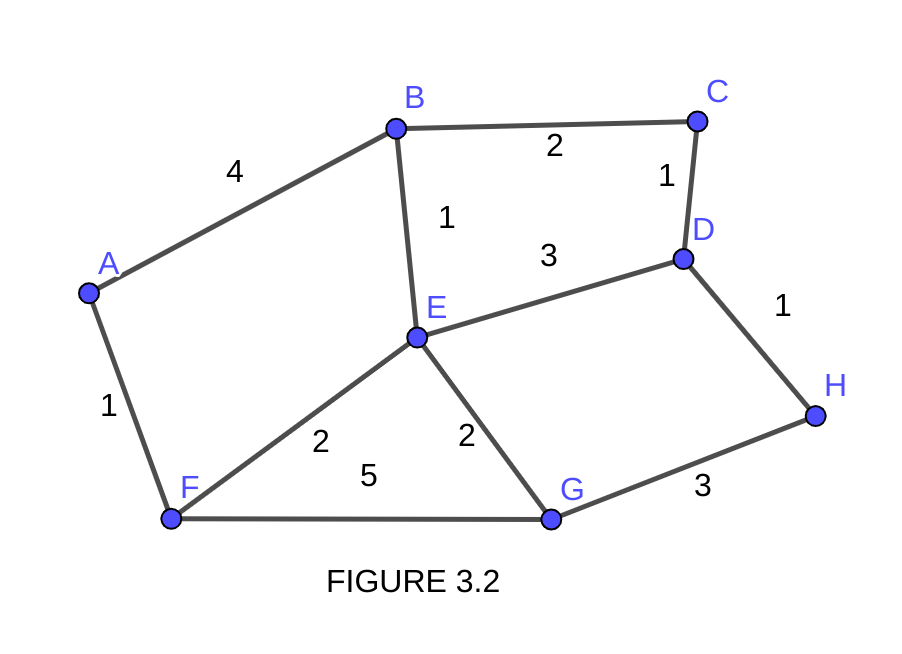
\includegraphics[width=0.5\columnwidth]{Figure3.2.png} % Example image
\end{center}

\subsection*{Réponse}Au premier, il faut trouver les sommets qui degre est impair. Donc on a sommet F, B, G, D. Ensuite on construire le Figure 3.2a\\

\begin{center}
	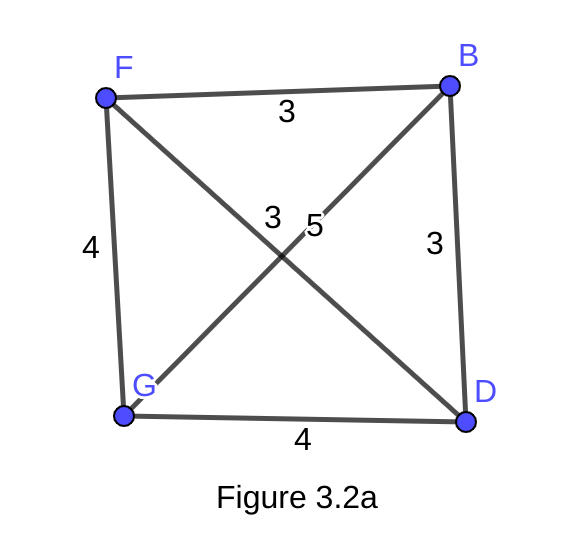
\includegraphics[width=0.5\columnwidth]{Figure3.2a.png} % Example image
\end{center}

Selon le Figure 3.2a, on veut connecter les 4 sommets avec le minimal poid, on peut choisir Edge(F, G) et Edge(B, D).\\

On peut ajouter un Edge(B, D) dans le Figure 3.2, donc il y a seulement 2 sommets impaire, on peut trouver un chemin eulerien.\\

Le poids minimal total est l'addition de tous les poids de Figure3.2 et Edge(F,G), Edge(B,D).\\

Tous les poids de Figure3.2 : \(1+4+2+1+1+3+2+2+5+1+3 = 25\)\\
Avec les 2 autre edges : \(25 + 3 + 4 = 32\)\\

Donc le poids minimal total est \textbf{32}.

\newpage

\section*{Question 1}

\begin{problem}
	What is the airspeed velocity of an unladen swallow?
\end{problem}
\begin{center}
	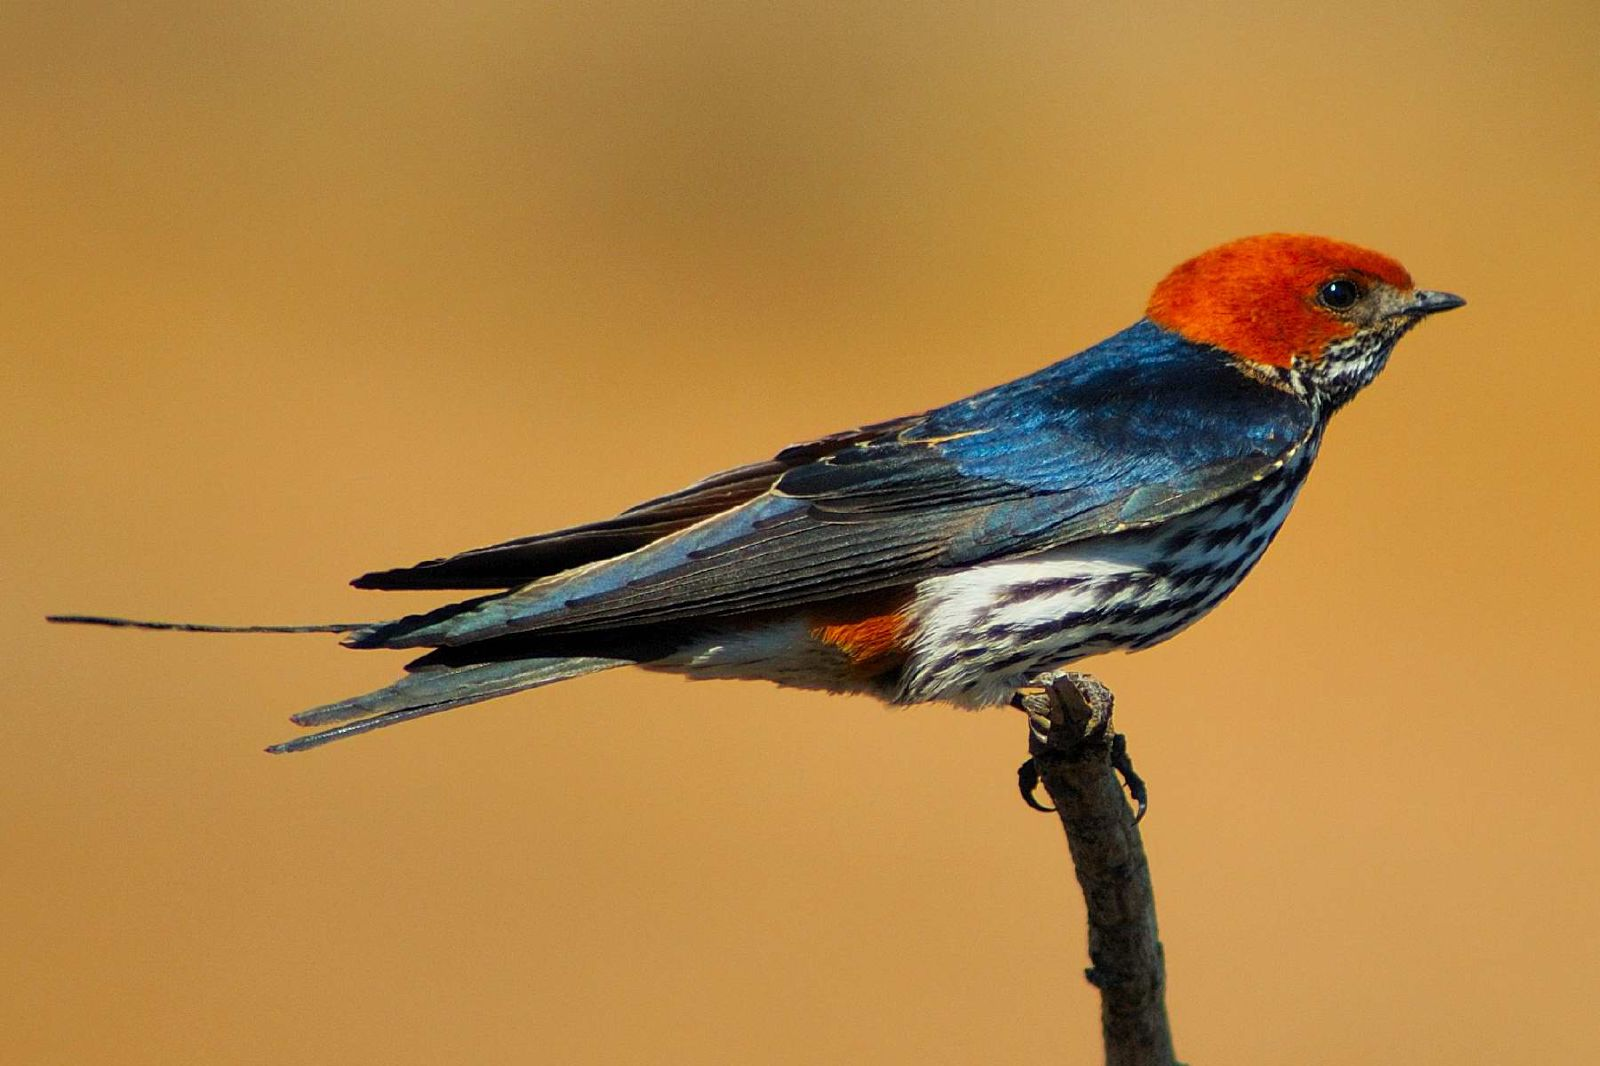
\includegraphics[width=0.5\columnwidth]{swallow.jpg} % Example image
\end{center}

%------------------------------------------------

\subsection*{Answer}

While this question leaves out the crucial element of the geographic origin of the swallow, according to Jonathan Corum, an unladen European swallow maintains a cruising airspeed velocity of \textbf{11 metres per second}, or \textbf{24 miles an hour}. The velocity of the corresponding African swallows requires further research as kinematic data is severely lacking for these species.

%----------------------------------------------------------------------------------------

\section*{Question 2}

\begin{problem}
	How much wood would a woodchuck chuck if a woodchuck could chuck wood?
	
	\medskip
	
	\begin{enumerate}[(\itshape a\normalfont)] % Sub-questions styled as italic letters
		\item Suppose ``chuck" implies throwing.
		\item Suppose ``chuck" implies vomiting.
	\end{enumerate}
\end{problem}

%------------------------------------------------

\subsection*{Answer}

\begin{enumerate}[(\itshape a\normalfont)] % Sub-questions styled as italic letters
	\item According to the Associated Press (1988), a New York Fish and Wildlife technician named Richard Thomas calculated the volume of dirt in a typical 25--30 foot (7.6--9.1 m) long woodchuck burrow and had determined that if the woodchuck had moved an equivalent volume of wood, it could move ``about \textbf{700 pounds (320 kg)} on a good day, with the wind at his back".
    
	\item A woodchuck can ingest 361.92 cm\textsuperscript{3} (22.09 cu in) of wood per day. Assuming immediate expulsion on ingestion with a 5\% retainment rate, a woodchuck could chuck \textbf{343.82 cm\textsuperscript{3}} of wood per day.
\end{enumerate}

%----------------------------------------------------------------------------------------

\section*{Question 3}

\begin{problem}
	Identify the author of Equation \ref{eq:bayes} below and briefly describe it in Latin.
	
	\medskip
	
	\begin{equation}\label{eq:bayes}
		P(A|B) = \frac{P(B|A)P(A)}{P(B)}
	\end{equation}
	
	\smallskip
\end{problem}

%------------------------------------------------

\subsection*{Answer} 

Lorem ipsum dolor sit amet, consectetur adipiscing elit. Praesent porttitor arcu luctus, imperdiet urna iaculis, mattis eros. Pellentesque iaculis odio vel nisl ullamcorper, nec faucibus ipsum molestie. Sed dictum nisl non aliquet porttitor. Etiam vulputate arcu dignissim, finibus sem et, viverra nisl. Aenean luctus congue massa, ut laoreet metus ornare in. Nunc fermentum nisi imperdiet lectus tincidunt vestibulum at ac elit. Nulla mattis nisl eu malesuada suscipit.

%----------------------------------------------------------------------------------------

\section*{Question 4 (bonus marks)}

\begin{problem}
	The table below shows the nutritional consistencies of two sausage types. Explain their relative differences given what you know about daily adult nutritional recommendations.
	
	\bigskip
    
	\begin{center}
		\begin{tabular}{l l l}
			\toprule
			\textit{Per 50g} & Pork & Soy \\
			\midrule
			Energy & 760kJ & 538kJ\\
			Protein & 7.0g & 9.3g\\
			Carbohydrate & 0.0g & 4.9g\\
			Fat & 16.8g & 9.1g\\
			Sodium & 0.4g & 0.4g\\
			Fibre & 0.0g & 1.4g\\
			\bottomrule
		\end{tabular}
	\end{center}
	
	\medskip
\end{problem}

%------------------------------------------------

\subsection*{Answer}

Lorem ipsum dolor sit amet, consectetur adipiscing elit. Praesent porttitor arcu luctus, imperdiet urna iaculis, mattis eros. Pellentesque iaculis odio vel nisl ullamcorper, nec faucibus ipsum molestie. Sed dictum nisl non aliquet porttitor. Etiam vulputate arcu dignissim, finibus sem et, viverra nisl. Aenean luctus congue massa, ut laoreet metus ornare in. Nunc fermentum nisi imperdiet lectus tincidunt vestibulum at ac elit. Nulla mattis nisl eu malesuada suscipit.

%----------------------------------------------------------------------------------------

\section*{Question 5 (bonus marks)}

\begin{problem}
	\lstinputlisting[
		caption=Luftballons Perl Script, % Caption above the listing
		label=lst:luftballons, % Label for referencing this listing
		language=Perl, % Use Perl functions/syntax highlighting
		frame=single, % Frame around the code listing
		showstringspaces=false, % Don't put marks in string spaces
		numbers=left, % Line numbers on left
		numberstyle=\tiny, % Line numbers styling
	]{luftballons.pl}
	
	\begin{enumerate}
		\item How many luftballons will be output by the Listing \ref{lst:luftballons} above?
		\item Identify the regular expression in Listing \ref{lst:luftballons} and explain how it relates to the anti-war sentiments found in the rest of the script.
	\end{enumerate}

\end{problem}

%------------------------------------------------

\subsection*{Answer}

\begin{enumerate}
	\item 99 luftballons.
	\item Lorem ipsum dolor sit amet, consectetur adipiscing elit. Praesent porttitor arcu luctus, imperdiet urna iaculis, mattis eros. Pellentesque iaculis odio vel nisl ullamcorper, nec faucibus ipsum molestie. Sed dictum nisl non aliquet porttitor. Etiam vulputate arcu dignissim, finibus sem et, viverra nisl. Aenean luctus congue massa, ut laoreet metus ornare in. Nunc fermentum nisi imperdiet lectus tincidunt vestibulum at ac elit. Nulla mattis nisl eu malesuada suscipit.
\end{enumerate}

%----------------------------------------------------------------------------------------

\end{document}
